\section{}



\subsection{}

Wir plotten zunächst die beiden Funktionen:

\lstinputlisting[style=pythoncode, linerange={1-3, 5-12}]{chapter_04/exercise_04_15.py}

Wir erhalten den folgenden Graphen:

\begin{center}
  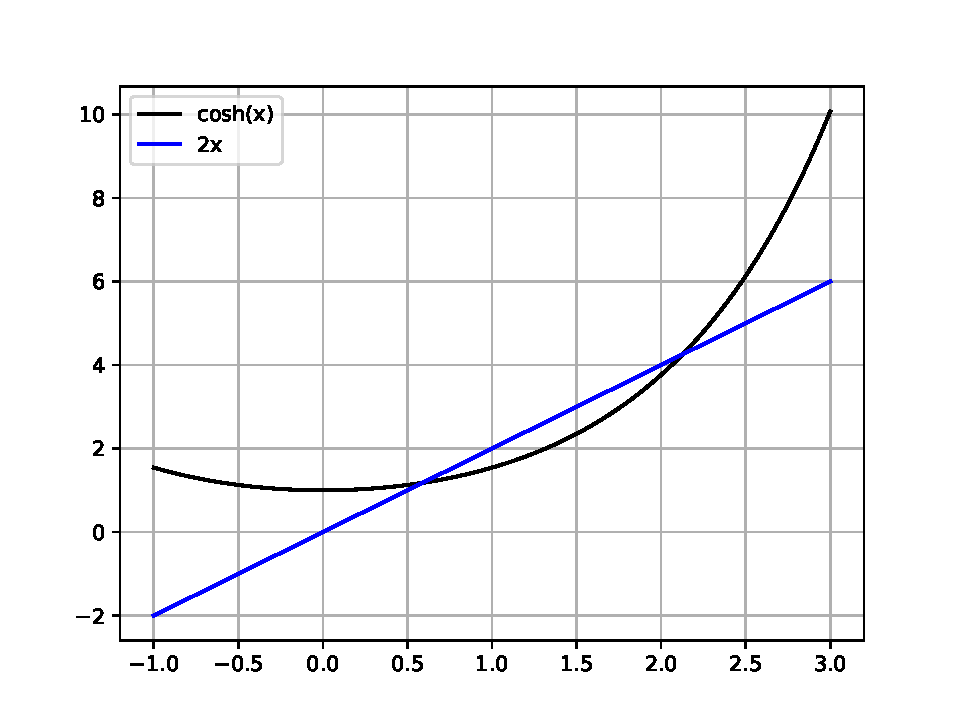
\includegraphics[width = 0.65\textwidth]{chapter_04/exercise_04_15_figure.pdf}
\end{center}

Wir bestimmen nun die beiden Nullstellen mit dem folgenden Code:

\lstinputlisting[style=pythoncode, firstline = 14, lastline = 19]{chapter_04/exercise_04_15.py}

Wir erhalten den folgenden Output:

\begin{consoleoutput}
  $ python exercise_04_15.py
  The intersections are at 0.5893877634693506 and 2.1267998926782568.
\end{consoleoutput}



\subsection{}

Die gegebene Funktion $f$ ist konvex;
für einen beliebigen Startwert $x_0$ mit $f'(x_0) \neq 0$ konvergiert daher das Newton-Verfahren gegen eine der beiden Nullstellen.
Der einzige krtische Punkt ist daher der Wert $x \in \Real$ mit $f'(x) = 0$ (dieser ist eindeutig, da $f$ als konvexe Funktion nur ein Minimum besitzen kann).
Wir bestimmen diesen Wert näherungsweise:

\lstinputlisting[style=pythoncode, firstline = 23, lastline = 24]{chapter_04/exercise_04_15.py}

Wir erhalten das folgende Ergebnis:

\begin{consoleoutput}
  The intersections are at 0.5893877634693506 and 2.1267998926782568.
\end{consoleoutput}
